\section{Evaluation: \nanomaly}
\label{sec:evaluation-nanomaly}
We have not really (\ES{huh?}) evaluated our prototype of \nanomaly in two phases:
%
\begin{enumerate}
\item We investigate the \emph{complexity} of the generated traces by various size metrics.
\item We investigate the \emph{usefulness} of the generated traces compared to the standard compiler errors by performing an A/B study.
\end{enumerate}

\subsection{Trace Complexity}
\label{sec:trace-complexity}
For each of the ill-typed programs from \S~\ref{sec:eval-witness} for
which we could find a witness, we measure the complexity of the
generated trace according to the following metrics:
%
\begin{enumerate}
\item The number of single-step reductions along the path from the
  witness to the stuck term. This can be thought of as a worst-case
  complexity, \ie ``How big is the fully-expanded trace?''
\item The number forward (or backward) jumps that can be taken along the
  path from the witness to the stuck term. These abstract many details
  of the computation that are often uninteresting or irrelevant to the
  explanation.
\item \ES{others?}
\end{enumerate}
%
\begin{figure}[t]
\centering
  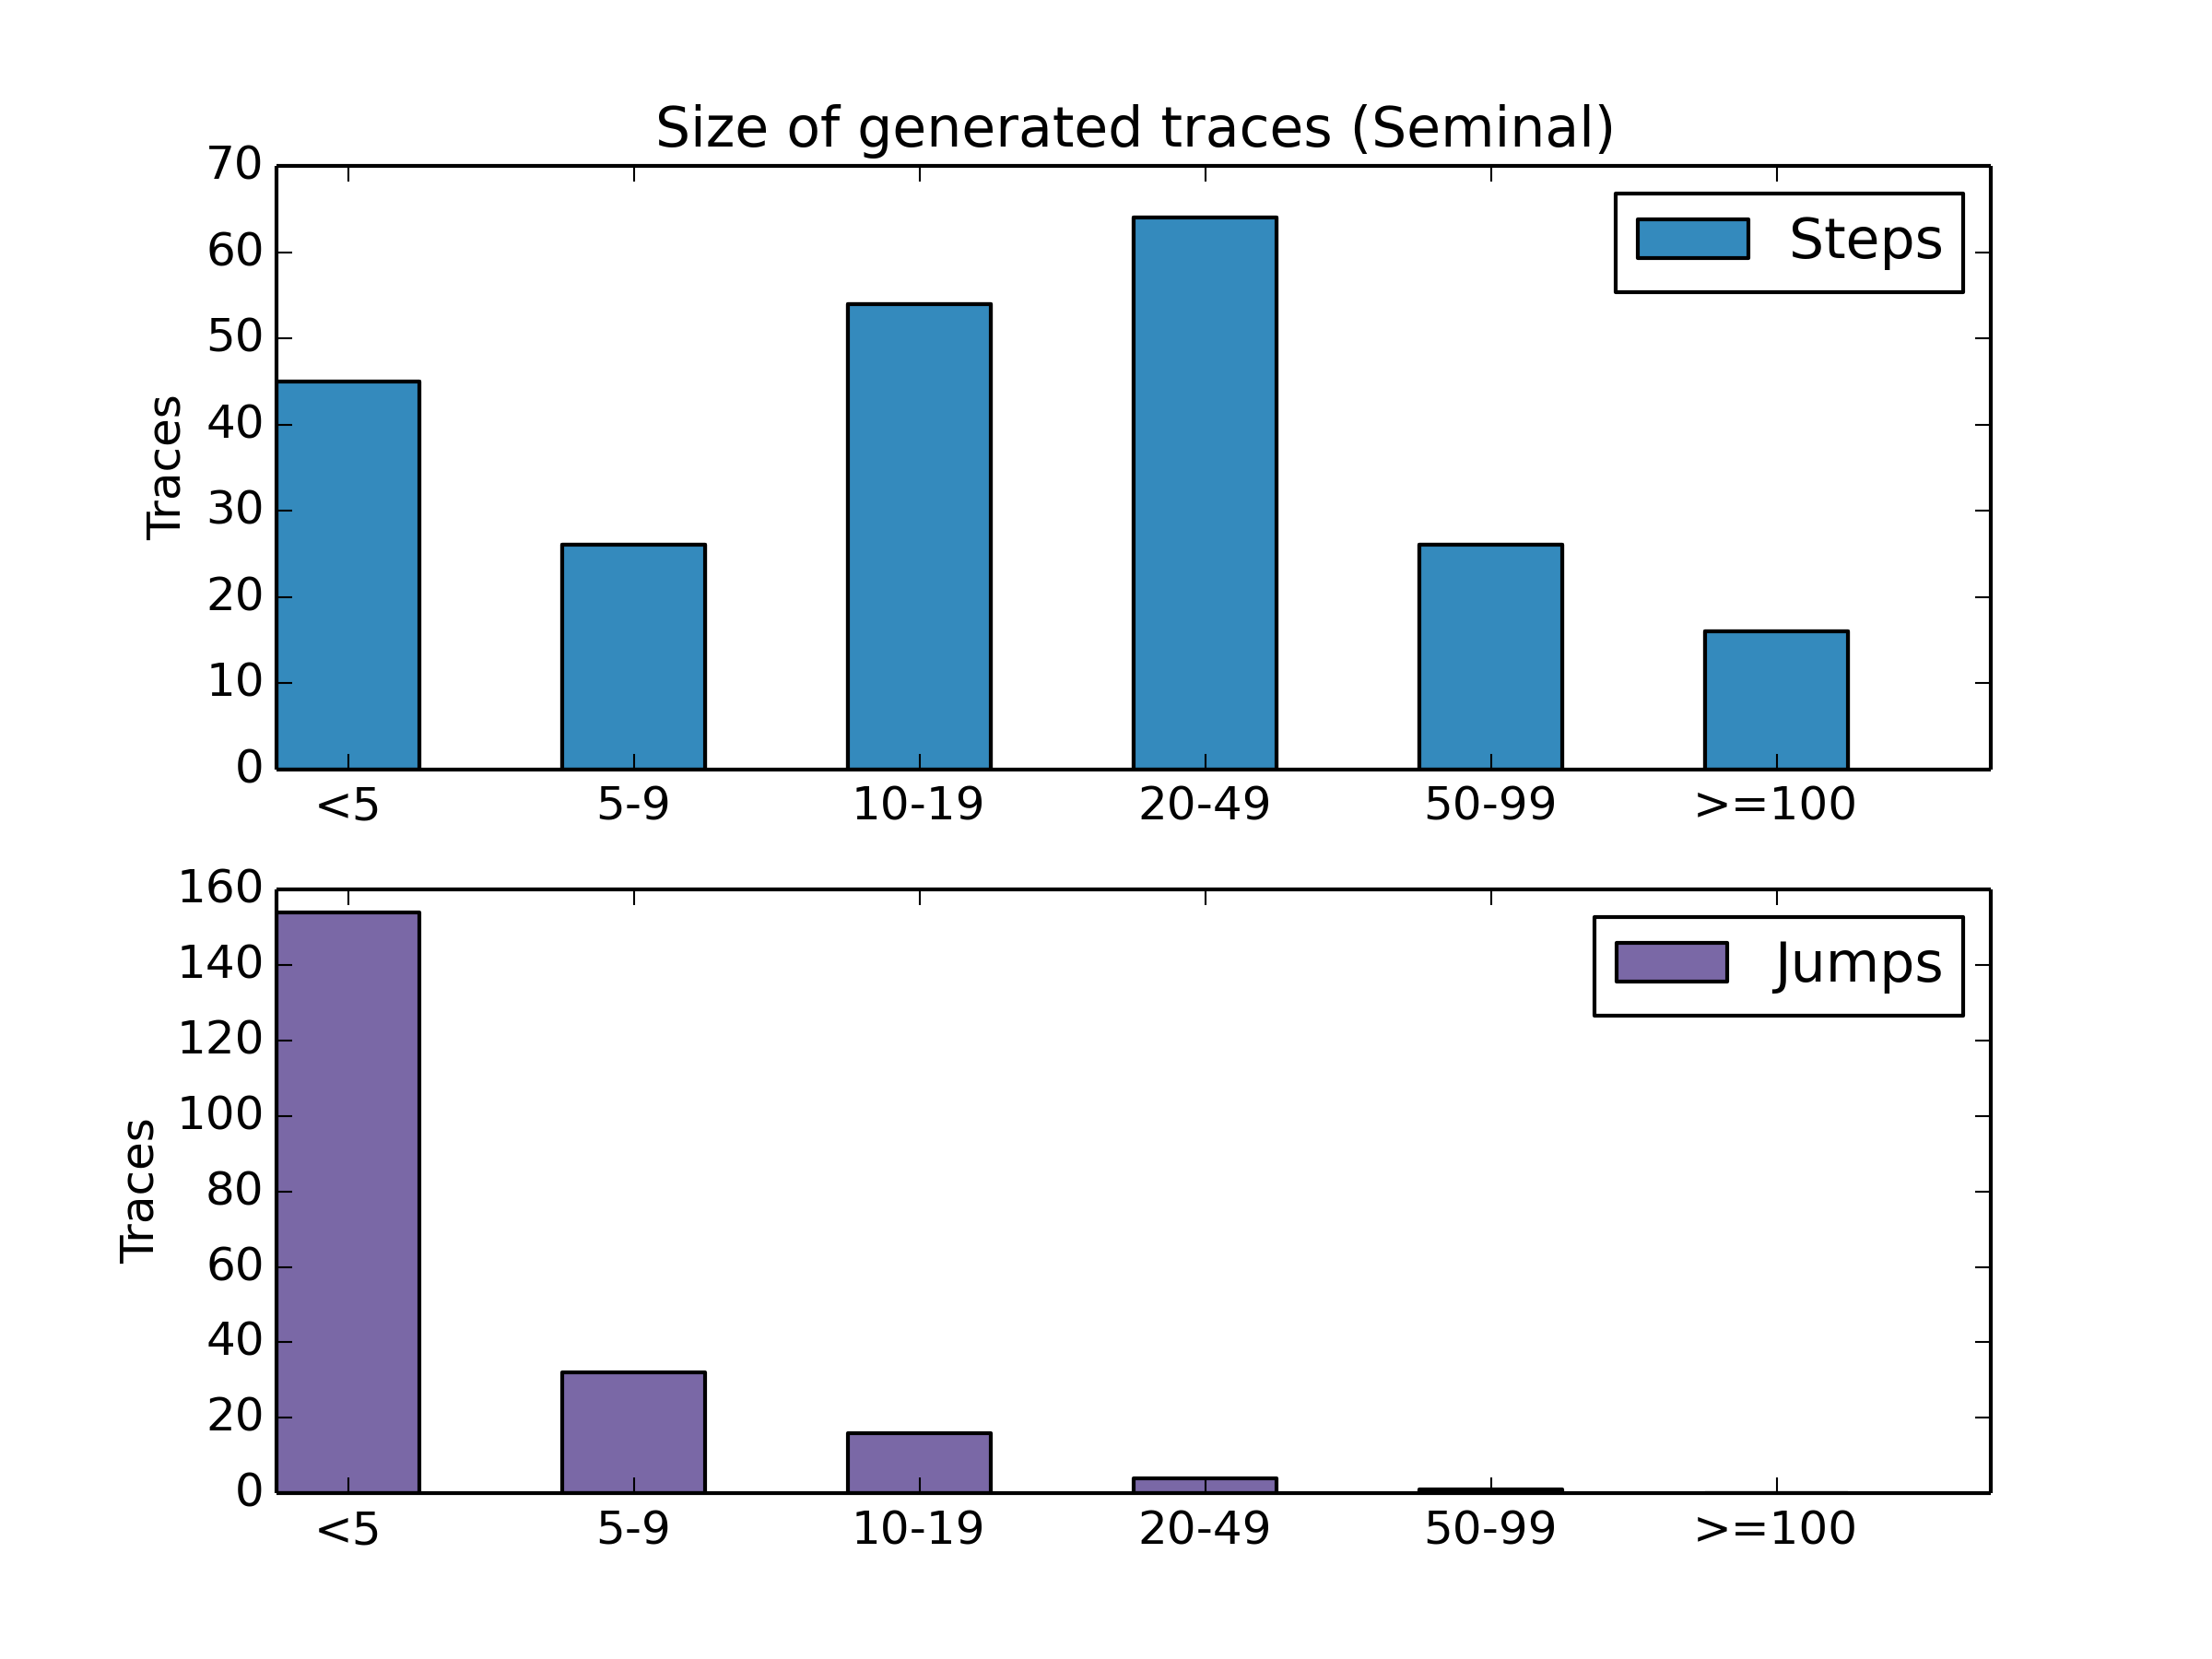
\includegraphics[width=\linewidth]{trace_size_seminal.png}
\caption{Complexity of the generated traces.}
\label{fig:results-complexity}
\end{figure}
%
The results of the experiment are summarized in
Figure~\ref{fig:results-complexity}.
%
The average number of single-step reductions is XX with a minimum of XX
and a maximum of XX. The average number of jumps is YY with a minimum of
YY and a maximium of YY.

\subsection{User Study}
\label{sec:user-study}
We also performed an A/B study at the University of Virginia (IRB
\#XXXX). 
%
Participants were recruited from the graduate-level Programming
Languages course CSYYY, with the possibility of winning a \$50 gift
certificate upon completion.
%
We selected a random sample of nine ill-typed programs from our
benchmark dataset and from submissions to our public-facing demo of
\nanomaly.
%
For each program, we presented participants with the program and
alternatingly, either \ocaml's type error message or our interactive
visualization of a preset trace.
%
In order to alleviate any potential bias in problem selection, we also
alternated whether participants began with \ocaml or \nanomaly.
%
Participants were asked to identify the \emph{source} of the error,
\emph{explain} the error, and finally \emph{fix} it.

We collected the time taken for each problem and recruited a colleague
to grade the submissions, hiding whether a given solution came from the
\ocaml or \nanomaly group.

\paragraph{Results}
\label{sec:study-results}
\ES{TODO!}
